\documentclass[10pt,twocolumn,letterpaper]{article}

\usepackage[letterpaper,textwidth=6.875in,textheight=8.875in,columnsep=0.3125in,top=1.0in]{geometry}
\usepackage{times}
\usepackage{amsmath,amssymb,amsfonts}
\usepackage{graphicx}
\usepackage{booktabs}
\usepackage{multirow}
\usepackage{xcolor}
\usepackage{microtype}
\usepackage{hyperref}
\usepackage{caption}
\usepackage{enumitem}
\usepackage{algorithm}
\usepackage{algorithmic}
\usepackage{titlesec}
\usepackage{fancyhdr}
\usepackage[switch,columnwise]{lineno}

\titlespacing*{\section}{0pt}{5.5pt plus 1pt minus 1pt}{2.2pt plus 0.5pt}
\titlespacing*{\subsection}{0pt}{4.2pt plus 0.8pt minus 0.8pt}{1.6pt plus 0.4pt}
\titlespacing*{\paragraph}{0pt}{2.6pt plus 0.4pt minus 0.4pt}{0.5em}

\hypersetup{
  colorlinks=true,
  linkcolor=blue!55!black,
  citecolor=blue!55!black,
  urlcolor=blue!55!black,
  pdftitle={Parts Before Points: Chirality-Free Anatomical Part Segmentation and Zero-Label Self-Distillation for Sim-to-Real Multi-Animal Pose Estimation},
  pdfauthor={Anonymous}
}

% CVPR-style double-blind review header & line numbers
\pagestyle{fancy}
\fancyhf{}
\renewcommand{\headrulewidth}{0pt}
\fancyhead[C]{\small\color{gray!70!black}CVPR 2026 CV4Animals Workshop Submission \#****.\quad CONFIDENTIAL REVIEW COPY.}
\fancyfoot[C]{\small\thepage}
\fancypagestyle{plain}{%
  \fancyhf{}
  \renewcommand{\headrulewidth}{0pt}
  \fancyhead[C]{\small\color{gray!70!black}CVPR 2026 CV4Animals Workshop Submission \#****.\quad CONFIDENTIAL REVIEW COPY.}
  \fancyfoot[C]{\small\thepage}
}
\renewcommand\linenumberfont{\normalfont\scriptsize\sffamily\color{cyan!65!black}}
\setlength\linenumbersep{6pt}

\captionsetup{font=footnotesize,labelfont=bf,skip=2.5pt}
\setlength{\textfloatsep}{6pt plus 1.5pt minus 1.5pt}
\setlength{\dbltextfloatsep}{7pt plus 1.5pt minus 1.5pt}
\setlength{\floatsep}{5pt plus 1.5pt minus 1.5pt}
\setlength{\intextsep}{5pt plus 1.5pt minus 1.5pt}
\renewcommand{\topfraction}{0.92}
\renewcommand{\dbltopfraction}{0.92}
\renewcommand{\textfraction}{0.07}

\title{\vspace{-2.2em}\Large\textbf{Parts Before Points: Chirality-Free Anatomical Part Segmentation\\and Zero-Label Self-Distillation for Sim-to-Real\\Multi-Animal Pose Estimation}\vspace{-0.6em}}

\author{
  Anonymous CV4Animals Submission\\
  \small Paper ID ****
}
\date{\vspace{-1.6em}}

\begin{document}
\linenumbers
\raggedbottom
\maketitle
\thispagestyle{plain}

\setlength{\abovedisplayskip}{4pt}
\setlength{\belowdisplayskip}{4pt}

\begin{abstract}
\vspace{-0.45em}
Markerless multi-animal pose estimation in behavioral neuroscience typically requires costly manual keypoint labeling whenever camera geometry, fur contrast, lighting, or cranial implants (headstages, miniscopes, tethers) change. Synthetic 3D rodent simulation offers a zero-annotation alternative, yet directly regressing keypoints from synthetic renders degrades sharply on real footage due to (i) local texture overfitting around discrete landmarks and (ii) \emph{chirality entanglement}, where predicting left/right points couples mirror-sensitive labels to hardware-occluded appearance cues. We propose \textbf{Parts Before Points}, a sim-to-real paradigm decoupling pose estimation into \emph{chirality-free anatomical body-part segmentation} (\texttt{head}, \texttt{snout}, \texttt{ear}, \texttt{torso}, \texttt{tail}) followed by a \emph{scale-invariant, occlusion-aware geometric pose solver} that resolves left/right handedness analytically from the spine vector. We instantiate this principle in single-frame \texttt{YOLO11n-seg} and a 580\,KB temporal VOS head (\texttt{Cutie-BodyPartSeg}), and introduce: (1) \textbf{Parts2Points-Distill}, a zero-label transductive cross-paradigm self-distillation framework transferring anatomy-gated unlabeled real poses into a 38\,FPS keypoint student; and (2) \textbf{Zero-GT-Seed Hybrid VOS Fusion}, which seeds frame 0 and re-anchors dark-corner drift purely from zero-shot part detections. On real CalMS21/MARS tethered footage (\texttt{mouse083}, 4,881 frames), zero-shot part segmentation cuts median error by \textbf{34.4\%} (22.34 $\to$ 14.66\,px) and lifts PCK@16 by \textbf{+20.1\,pts}. Zero-label \textbf{Parts2Points-Distill} cuts RMSE \textbf{50.0\%} (54.31 $\to$ 27.20\,px, $p=3.66\times 10^{-23}$), collapses L/R swaps \textbf{8.4$\times$} (12.46\% $\to$ 1.48\%), and decisively beats a same-paradigm \textbf{Points2Points-Distill} control ($p=1.90\times 10^{-24}$), proving cross-paradigm part supervision breaks self-training confirmation bias. On an unseen second real rig (\texttt{OFT\_54}, $192\times 192$, 0 target labels/tuning), \textbf{Parts2Points-Distill} transfers inductively at \textbf{97.0\%} recall and \textbf{4.33\,px} (9.3\% body-length) centroid error, while \textbf{Zero-GT-Seed Hybrid Fusion} outperforms 20-real-label active learning on dyadic nose-to-nose correlation ($r=0.936$ vs.\ $0.875$) and social contact F1 ($0.814$ vs.\ $0.739$).
\end{abstract}

% =========================================================================
\section{Introduction}
% =========================================================================

Quantitative behavioral neuroscience relies on markerless multi-animal pose tracking to measure social investigation, aggression, grooming, and neural-behavioral coupling~\cite{mathis2018deeplabcut,pereira2022sleap,segalin2021mars,sun2021calms21}. Modern keypoint estimators~\cite{mathis2018deeplabcut,pereira2022sleap,jocher2023ultralytics} excel given hundreds of manually labeled target-rig frames, yet real experiments undergo severe visual shifts: bright white cranial headstages and dark fiber-optic tethers bisect black C57BL/6 mice, white BALB/c intruders blend into wood-shaving bedding, dark arena corners swallow silhouettes, and different rigs vary widely in resolution and illumination.

Parametric 3D animal simulation generates pixel-exact supervision across arbitrary viewpoints and behaviors at zero labeling cost~\cite{bolanos2021three,dunn2021geometric}. However, training a direct keypoint detector (\texttt{YOLO11n-pose}) solely on 3D simulated two-mouse footage and evaluating zero-shot on real CalMS21/MARS footage (\texttt{mouse083\_task1\_annotator1.mp4}) yields severe degradation: median error 22.34--31.05\,px, left/right swap rate 12.5--27.8\%, and tethered-mouse PCK@16 of just 15.2\%.

\begin{figure*}[t]
  \centering
  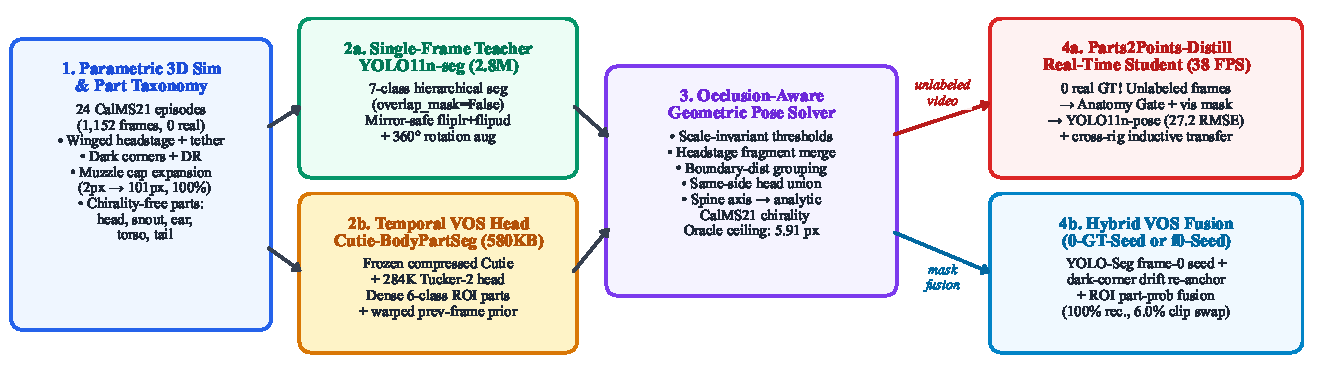
\includegraphics[width=0.92\textwidth]{figures/fig1_pipeline.pdf}
  \caption{\textbf{Overview of the \emph{Parts Before Points} framework.} (1) Parametric 3D CalMS21 simulation generates synchronized YOLO-Seg, COCO-Seg, and packed 6-class semantic part masks with anterior rhinarium muzzle expansion (0 real labels). (2) Chirality-free part segmentation is instantiated across single-frame \texttt{YOLO11n-seg} (\texttt{overlap\_mask=False}) and a 580\,KB Tucker-2 temporal VOS head (\texttt{Cutie-BodyPartSeg}). (3) A scale-invariant, occlusion-aware geometric solver merges headstage-split fragments and resolves CalMS21 chirality analytically from the spine axis (5.91\,px oracle ceiling). (4a) \textbf{Parts2Points-Distill} distills anatomy-gated unlabeled real poses into a 38\,FPS student that also transfers inductively to unseen rigs. (4b) \textbf{Hybrid VOS Part Fusion} uses zero-shot \texttt{YOLO11n-seg} to seed frame 0, re-anchor dark-corner drift, and fuse ROI part probabilities.}
  \label{fig:pipeline}
\end{figure*}

Our error analysis isolates two structural flaws in direct keypoint regression under sim-to-real shift:
\begin{enumerate}[leftmargin=*,itemsep=1pt,topsep=1.5pt]
  \item \textbf{Point-texture fragility:} Keypoint heads depend on local intensity gradients around discrete 2D coordinates; synthetic fur shading, sensor noise, and unmodeled cranial hardware disrupt those local cues even when global body shape is clear.
  \item \textbf{Chirality entanglement:} Predicting \texttt{left\_ear} vs.\ \texttt{right\_ear} (or hips) directly forces a convolutional head to jointly localize a landmark and infer global 2D orientation. Under headstage occlusion, direct Sim v3 inverts left/right identity on 20.7\% of tethered resident frames.
\end{enumerate}

We propose \textbf{Parts Before Points} (Figure~\ref{fig:pipeline}), grounded in a geometric observation: \emph{anatomical body parts (\texttt{head}, \texttt{snout}, \texttt{ear}, \texttt{torso}, \texttt{tail}) are region-supported, shape-defined, and completely chirality-free.} Decoupling \emph{part semantics} from \emph{left/right handedness} unlocks full mirror-invariant augmentation (\texttt{fliplr}, \texttt{flipud}, $360^\circ$ rotation), anchors posterior landmarks on robust silhouettes, and resolves chirality analytically from the spine vector.

To keep adaptation regimes explicit, we evaluate three settings: (i) \emph{zero-shot cross-domain} transfer (synthetic training only), (ii) \emph{zero-label transductive self-distillation} on strictly disjoint unlabeled target frames (\textbf{Parts2Points-Distill}, 38\,FPS), and (iii) \emph{zero-label inductive cross-rig transfer} testing the distilled student untouched on a second real open-field rig (\texttt{OFT\_54}, $192\times 192$). A controlled same-paradigm baseline (\textbf{Points2Points-Distill}) proves direct-pose self-training stalls under confirmation bias, whereas cross-paradigm part-to-point distillation breaks through to near-supervised accuracy.

\paragraph{Contributions.}
\begin{enumerate}[leftmargin=*,itemsep=0.5pt,topsep=1.5pt]
  \item \textbf{Chirality-free body-part segmentation for pose:} Multi-format body-part dataset with rhinarium muzzle expansion (100\% snout yield, 5.91\,px oracle ceiling), yielding large zero-shot gains on both \texttt{YOLO11n-seg} (-34.4\% p50, +20.1\,pts PCK@16) and a 580\,KB temporal VOS head \texttt{Cutie-BodyPartSeg} (5.7$\times$ OKS AP50 over \texttt{Cutie-Pose}, 10.05\,px resident p50).
  \item \textbf{Scale-invariant, occlusion-aware part-to-pose geometry:} Parent fragment merging, scale-relative boundary grouping, and same-side head union cut real nose error 72.4\% (58.23 $\to$ 16.10\,px) with zero retraining and transfer from $1024\times 570$ to $192\times 192$.
  \item \textbf{Cross-paradigm \texttt{Parts2Points-Distill} (0 real labels, 38\,FPS):} Surpasses its own segmentation teacher ($p=1.74\times 10^{-11}$), cuts RMSE 50.0\% and swaps 8.4$\times$ vs.\ Sim v3 ($p=3.66\times 10^{-23}$), beats same-paradigm \texttt{Points2Points-Distill} ($p=1.90\times 10^{-24}$), and transfers inductively to unseen \texttt{OFT\_54} at 97.0\% recall and 4.33\,px centroid error.
  \item \textbf{Zero-GT-Seed Hybrid VOS Fusion:} Seeding Cutie frame 0 purely from zero-shot \texttt{YOLO11n-seg} plus dark-corner drift re-anchoring achieves 100\% clip recall, 15.02\,px p50, and beats 20-real-label active learning on dyadic nose-to-nose correlation ($r=0.936$) and contact F1 ($0.814$).
\end{enumerate}

% =========================================================================
\section{Related Work}
% =========================================================================

\paragraph{Markerless Multi-Animal Pose Estimation.} DeepLabCut~\cite{mathis2018deeplabcut,lauer2022multi}, SLEAP~\cite{pereira2022sleap}, MARS~\cite{segalin2021mars}, and YOLO-Pose~\cite{jocher2023ultralytics} achieve strong accuracy given hundreds of manual labels. Foundation models like SuperAnimal~\cite{ye2024superanimal} pool large labeled multi-species corpora for cross-lab inference, yet still regress chiral keypoints directly and degrade under lab-specific headstages or unfamiliar IR contrast without fine-tuning. Shifting the intermediate representation to chirality-free anatomical parts is orthogonal and adapts from unlabeled video alone.

\paragraph{Sim-to-Real Animal Pose and 3D Modeling.} Synthetic rodent renders~\cite{bolanos2021three,dunn2021geometric,karashchuk2021anipose} and domain randomization~\cite{tobin2017domain} reduce manual labeling, yet bridging synthetic shading to real IR home-cage recordings with cranial implants remains difficult for direct keypoint regressors. Benchmarking three progressive simulation generations shows that shifting supervision from points to anatomical parts yields larger zero-shot gains than appearance randomization alone.

\paragraph{VOS and Cross-Paradigm Self-Distillation.} Memory-based VOS trackers like CUTIE~\cite{cheng2024putting} maintain object identities across occlusions via object-level transformer memory. We pair a frozen Tucker-2 compressed CUTIE backbone with $\sim$580\,KB per-object heads to compare direct keypoint heatmaps against dense body-part decoding at matched capacity. For domain adaptation, naive keypoint self-training~\cite{xie2020self,sohn2020fixmatch,ye2024superanimal} suffers confirmation bias on mirrored or collapsed skeletons; our controlled \texttt{Points2Points-Distill} vs.\ \texttt{Parts2Points-Distill} study isolates how cross-paradigm part teachers plus anatomical gating eliminate this failure mode.

% =========================================================================
\section{Method}
% =========================================================================

\subsection{Parametric 3D Simulation and Chirality-Free Taxonomy}
\label{sec:dataset}

We generate synthetic two-mouse data via a Three.js physics simulator extended with CalMS21-calibrated rig anchors (\texttt{nose}, \texttt{left\_ear}, \texttt{right\_ear}, \texttt{neck}, \texttt{left\_hip}, \texttt{right\_hip}, \texttt{tail\_base}), 3D winged and tall-miniscope cranial headstages, flexible dark tethers, and low-illumination corner-huddling episodes. Rendering 24 episodes (20 train / 4 val, 48 frames each $\to$ 960 train / 192 val frames at $768\times 428$) with randomized contrast, gamma, vignetting, blur, sensor noise, and JPEG compression yields pixel-exact \texttt{(track\_id, part\_id)} masks and 3D keypoints at zero annotation cost.

\paragraph{Chirality-Free Semantic Part Space.} Rather than encoding left/right pixels, we map 11 raw 3D mesh parts into 6 canonical semantic classes:
{\small
\begin{equation}
  \mathcal{C}_{\text{sem}} = \{\texttt{0:bg},\, \texttt{1:head},\, \texttt{2:snout},\, \texttt{3:ear},\, \texttt{4:torso},\, \texttt{5:tail}\},
\end{equation}}
folding both pinnae into \texttt{ear} and neck/limbs into \texttt{torso}. For single-frame hierarchical instance segmentation, we emit 7 classes:
{\small
\begin{equation}
  \begin{aligned}
    \mathcal{C}_{\text{hier}} = \{&\texttt{resident},\, \texttt{intruder},\, \texttt{head},\\
    &\texttt{snout},\, \texttt{ear},\, \texttt{torso},\, \texttt{tail}\},
  \end{aligned}
\end{equation}}
where parent silhouettes exclude the thin tail to keep bounding boxes tight, while \texttt{head} covers the union of skull, snout, and ears for hardware robustness. Because neither taxonomy has chiral labels, \texttt{fliplr}, \texttt{flipud}, and $360^\circ$ rotation are strictly label-preserving.

\paragraph{Anterior Rhinarium Muzzle Cap Expansion.} In raw $768\times 428$ renders, the rhinarium mesh (\texttt{snoutTip}) spans only 2--4\,px, causing 99.9\% (2,302/2,304) of \texttt{snout} polygons to fail contour area filters. Our \texttt{expand\_snout\_muzzle\_mask} operator dilates the rhinarium $M_{\text{tip}}$ inside $M_{\text{head}}$ using scale-adaptive radius
{\small
\begin{equation}
  r = \mathrm{clip}\!\left(0.42 \sqrt{\tfrac{4}{\pi}|M_{\text{head}} \cup M_{\text{tip}}|},\; 6,\; 14\right)\,\text{px},
\end{equation}}
falling back to the top 22\% anterior pixels of $M_{\text{head}}$ along $\mathbf{c}_{\text{head}}-\mathbf{c}_{\text{torso}}$ when self-occluded (2.3\% of frames). This raises snout yield to 100.0\% (2,304/2,304, median 101\,px) with pixel-aligned nose tips (1.91\,px oracle nose ceiling).

\subsection{Dual-Paradigm Body-Part Segmentation Models}
\label{sec:models}

\paragraph{Single-Frame Teacher (\texttt{YOLO11n-seg}).} Starting from COCO-pretrained \texttt{yolo11n-seg.pt} (2.84M params, 6.0\,MB), we fine-tune on 7-class Sim v3 for 18 epochs ($512\times 512$, batch 32, AdamW, $\mathrm{lr}_0=3\times 10^{-3}$, cosine schedule, \texttt{degrees}=180, \texttt{fliplr}=0.5, \texttt{flipud}=0.5). Crucially, we set \textbf{\texttt{overlap\_mask=False}}: because \texttt{head}, \texttt{snout}, \texttt{ear}, and \texttt{torso} lie inside parent masks, disabling exclusive rasterization prevents overlapping targets from erasing one another.

\paragraph{Temporal VOS Head (\texttt{Cutie-BodyPartSeg}) and Provenance.} We freeze a 31.7\,MB (15.76M-param) Conv+BN-folded, HOSVD Tucker-2 compressed CUTIE backbone (\texttt{cutie-sam3-bodyparts.pth}). Regarding pretraining provenance: this backbone was distilled from class-agnostic SAM\,3.1 + DINOv3 teachers purely for generic mask propagation and contains \emph{zero CalMS21/MARS mouse keypoint supervision}, paralleling COCO pretraining in \texttt{YOLO11n}. We tap per-object decoder features $\mathbf{F}_{p4}\in\mathbb{R}^{128\times H/4\times W/4}$ and $\mathbf{F}_{p8}\in\mathbb{R}^{128\times H/8\times W/8}$, sample $1.5\times$ padded square ROIs ($32\times 32$ features, $64\times 64$ RGB/mask), and warp $\mathbf{P}_{t-1}^{(o)}$ from $\mathrm{ROI}_{t-1}\to\mathrm{ROI}_t$. A 283,542-param (\textbf{580.2\,KB} fp16) Tucker-2 residual head fuses features, RGB (20\% dropout), tracked mask, and warped prior (45\% cold-start dropout) to emit $\mathbf{Z}_t^{(o)}\in\mathbb{R}^{6\times 64\times 64}$, trained 30 epochs with weighted cross-entropy plus foreground Soft Dice:
{\small
\begin{equation}
  \mathcal{L}_{\text{part}} = \mathcal{L}_{\text{WCE}}(\mathbf{Z}, \mathbf{Y}; \mathbf{w}) + 1.2\Big(1 - \tfrac{1}{5}\textstyle\sum_{c=1}^{5}\mathrm{Dice}(\mathbf{P}_c, \mathbf{Y}_c)\Big),
\end{equation}}
with $\mathbf{w}=[0.35, 1.2, 2.6, 2.8, 1.0, 2.2]$. For matched-capacity comparison, \texttt{Cutie-Pose} (284,534 params, 582.2\,KB fp16) uses the identical frozen backbone and head capacity to regress 7 DSNT keypoint heatmaps directly.

\subsection{Scale-Invariant, Occlusion-Aware Geometric Solver}
\label{sec:geometry}

Given per-animal part masks $\{M_{\text{head}}, M_{\text{snout}}, M_{\text{ear}}, M_{\text{torso}}, M_{\text{tail}}\}$ and optional parent mask $M_p$, our deterministic solver derives all 7 keypoints without learned coordinate bias. Defining each animal's characteristic scale $s_p = \max(24,\,\sqrt{|M_p|})$ makes all spatial thresholds scale-invariant across camera resolutions ($1024\times 570$ down to $192\times 192$):
\begin{enumerate}[leftmargin=*,itemsep=0.5pt,topsep=1.5pt]
  \item \textbf{Forward heading $\hat{\mathbf{u}}$:} Weighted vector voting combines $(\mathbf{c}_{\text{head}}-\mathbf{c}_{\text{torso}}, 3.5)$, $(\mathbf{c}_{\text{snout}}-\mathbf{c}_{\text{torso}}, 3.0)$, $(\mathbf{c}_{\text{snout}}-\mathbf{c}_{\text{head}}, 2.5)$, $(\mathbf{c}_{\text{torso}}-\mathbf{p}_{\text{tail\_prox}}, 2.2)$, and $(\bar{\mathbf{c}}_{\text{ear}}-\mathbf{c}_{\text{torso}}, 2.0)$, falling back to silhouette PCA disambiguated by $\hat{\mathbf{u}}_{t-1}$ only if all directional parts vanish.
  \item \textbf{Nose \& tail base:} $\mathbf{p}_{\text{nose}}$ is the mean of top 95th-percentile pixels of $M_{\text{snout}}$ (fallback $M_{\text{head}}$) along $+\hat{\mathbf{u}}$. $\mathbf{p}_{\text{tail\_base}}$ is the closest junction ($0.65\,\mathbf{p}_{\text{torso}}+0.35\,\mathbf{p}_{\text{tail}}$) between posterior 40\% of $M_{\text{torso}}$ and $M_{\text{tail}}$ within $0.75\,s_p$ (else 96th-percentile posterior extreme of $M_{\text{torso}}$).
  \item \textbf{Neck, analytic chirality, \& hips:} $\mathbf{p}_{\text{neck}} = 0.28\,\mathbf{e}_{82}(M_{\text{head}}, -\hat{\mathbf{u}}) + 0.72\,\mathbf{e}_{84}(M_{\text{torso}}, +\hat{\mathbf{u}})$. Defining $\hat{\mathbf{h}}=\mathrm{unit}(\mathbf{p}_{\text{nose}}-\mathbf{p}_{\text{neck}})$ and $\hat{\mathbf{t}}=\mathrm{unit}(\mathbf{p}_{\text{neck}}-\mathbf{p}_{\text{tail\_base}})$, CalMS21 image-plane chirality ($y$ down) satisfies $\det([\hat{\mathbf{h}}, \mathbf{p}_L - \mathbf{p}_R]) > 0$, giving exact left normal $\hat{\mathbf{n}}_L = (-\hat{h}_y, \hat{h}_x)$ to sort ear components. Hips lie at the 97th/3rd-percentile flanks of $M_{\text{torso}}$ at $\mathbf{p}_{\text{neck}}+0.62(\mathbf{p}_{\text{tail\_base}}-\mathbf{p}_{\text{neck}})$.
\end{enumerate}

\paragraph{Scale-Invariant Headstage-Aware Grouping and Schema Generality.} Bright white headstages often bisect black mice into a dark torso and detached anterior rostrum $>100$\,px from the torso centroid, causing naive centroid grouping to drop the head (58.23\,px nose error). We fix this via three scale-relative rules: (i) \emph{parent fragment merging} when a secondary same-class parent ($\le 0.65\times$ primary area) lies within $0.55\,s_p$ boundary distance (supporting both dyadic deduplication and arbitrary $N\ge 3$ same-class animals by suppressing duplicates with $\mathrm{IoU}\ge 0.45$ while assigning unique instance IDs); (ii) \emph{boundary-distance association} within $0.60\,s_p$ for anterior parts (\texttt{head}/\texttt{snout}/\texttt{ear}) and $0.45\,s_p$ for \texttt{tail} when containment $<0.10$; and (iii) \emph{same-side head union} merging anterior \texttt{head} fragments with $\langle \mathbf{c}_{h_0}-\mathbf{c}_{\text{torso}}, \mathbf{c}_{h_k}-\mathbf{c}_{\text{torso}}\rangle > 0$. The same geometric interface generalizes directly to non-rodent body plans (e.g., 3-tagma insect \texttt{head}/\texttt{thorax}/\texttt{abdomen} masks $\to$ 5 axial landmarks via distance-transform head-capsule and boundary-interface centroids).

\subsection{Zero-Label Cross-Paradigm Self-Distillation}
\label{sec:distill}

\begin{algorithm}[t]
\caption{\textbf{Parts2Points-Distill} (Zero Real Labels, 38\,FPS)}
\label{alg:p2p}
\footnotesize
\begin{algorithmic}[1]
\REQUIRE Sim part teacher $f_{\text{seg}}$, Sim v3 pose init $f_{\text{pose}}^{(0)}$, Sim replay $\mathcal{D}_{\text{sim}}$, disjoint unlabeled target frames $\mathcal{U}$
\STATE $\mathcal{P}_{\text{clean}} \leftarrow \emptyset$
\FORALL{unlabeled frame $I \in \mathcal{U}$}
  \STATE $\mathcal{M} \leftarrow f_{\text{seg}}(I)$;\quad $\hat{P} \leftarrow \mathrm{GeomPoseSolver}(\mathcal{M})$
  \IF{$\mathcal{G}_{\text{anat}}(\hat{P}) = \text{True}$}
    \STATE Set visibility $v_k \leftarrow 2\cdot\mathbb{I}[s_k \ge 0.72]$ for $k=1\dots 7$
    \STATE $\mathcal{P}_{\text{clean}} \leftarrow \mathcal{P}_{\text{clean}} \cup \{(I, \hat{P}, \mathbf{v})\}$
  \ENDIF
\ENDFOR
\STATE Sample $|\mathcal{P}_{\text{clean}}|$ replay frames $\mathcal{D}_{\text{rep}} \subset \mathcal{D}_{\text{sim}}$ (1:1 ratio)
\STATE $f_{\text{pose}} \leftarrow \mathrm{Train}(f_{\text{pose}}^{(0)},\; \mathcal{P}_{\text{clean}} \cup \mathcal{D}_{\text{rep}},\; \text{14 ep},\; \text{lr}_0=8\times 10^{-4})$
\RETURN Real-time keypoint student $f_{\text{pose}}$ (38\,FPS)
\end{algorithmic}
\end{algorithm}

Full-resolution \texttt{retina\_masks} decoding runs at 7.7\,FPS, whereas \texttt{YOLO11n-pose} runs at 38--45\,FPS. Algorithm~\ref{alg:p2p} bridges this speed-accuracy gap with zero real labels. The unsupervised \textbf{Anatomical Self-Consistency Gate} $\mathcal{G}_{\text{anat}}(\hat{P})$ accepts a dual-animal frame only if both mice satisfy: (a) parent conf $\ge 0.45$ and mask-grounded core landmarks ($s_{\text{nose}}, s_{\text{neck}} \ge 0.78$, $s_{\text{tail\_base}} \ge 0.70$); (b) spine length $L=\|\mathbf{p}_{\text{nose}}-\mathbf{p}_{\text{tail\_base}}\|\in[72, 270]$\,px and neck projection $\in[0.42, 0.86]L$; (c) non-kinked angle $\cos\angle(\hat{\mathbf{h}},\hat{\mathbf{t}})\ge -0.35$; (d) ear/hip span ratios $\in[0.10,0.55]/[0.16,0.68]$; (e) strict dual-axis CalMS21 chirality; and (f) centroid separation $\ge 38$\,px. Masking fallback keypoints ($s_k < 0.72 \Rightarrow v_k=0$) prevents noisy unsegmented pinnae from corrupting gradients while 1:1 Sim v3 replay preserves ear geometry.

\subsection{Zero-GT-Seed Hybrid VOS Part Fusion}
\label{sec:hybrid}

Standalone VOS trackers excel on continuous tethered trajectories (10.05\,px resident p50), yet need a frame-0 seed mask and can collapse in dark corners. \textbf{Zero-GT-Seed Hybrid VOS Part Fusion} removes manual seeding and drift with zero retraining: (i) on frame 0, zero-shot \texttt{YOLO11n-seg} predicts initial parent masks automatically (\textbf{0 human masks anywhere}); (ii) whenever Cutie's mask area drops below $0.48\times$ \texttt{YOLO11n-seg}'s parent area or $\mathrm{IoU} < 0.28$ (conf $\ge 0.45$, area $\ge 1200$\,px, 10-frame cooldown), the repaired mask is re-injected into Cutie's memory; and (iii) inside each $128\times 128$ decoding ROI, Cutie part probabilities linearly fuse with rasterized \texttt{YOLO11n-seg} masks ($w_{\text{yolo}}=\{0.55, 0.65, 0.50, 0.45, 0.75\}$ for \texttt{head}, \texttt{snout}, \texttt{ear}, \texttt{torso}, \texttt{tail}) prior to pose extraction.

% =========================================================================
\section{Experimental Setup}
% =========================================================================

\begin{table*}[t]
  \centering
  \caption{\textbf{Full-video 200-frame real benchmark on \texttt{mouse083\_task1\_annotator1.mp4} ($1024\times 570$, unified Hungarian matching).} Bracketed intervals denote 2,000-resample frame-cluster bootstrap 95\% CIs. \textbf{Bold} marks best 0-real-label result; * denotes 20-real-label supervised active learning. \texttt{Points2Points-Distill} is our same-paradigm control under the exact same 600-frame pool, gate, and 187-frame budget.}
  \label{tab:main_200f}
  \renewcommand{\arraystretch}{0.95}
  \resizebox{\textwidth}{!}{%
  \begin{tabular}{@{}llcccccccccccc@{}}
    \toprule
    \textbf{Method} & \textbf{Regime} & \textbf{Real} & \textbf{FPS} & \textbf{Rec.} & \textbf{Cls} & \textbf{RMSE} & \textbf{MAE} & \textbf{p50 [95\% CI]} & \textbf{p90} & \textbf{PCK@16} & \textbf{PCK@32} & \textbf{mOKS} & \textbf{Swap} \\
    & & \textbf{Lbls} & (M2) & (\%) & (\%) & (px) $\downarrow$ & (px) $\downarrow$ & (px) $\downarrow$ & (px) $\downarrow$ & (\%) $\uparrow$ & (\%) $\uparrow$ & $\uparrow$ & (\%) $\downarrow$ \\
    \midrule
    \emph{Oracle GT Part Masks $\to$ Pose} & \emph{Ceiling} & \emph{--} & \emph{--} & \emph{100} & \emph{100} & \emph{--} & \emph{6.21} & \emph{5.91} & \emph{10.28} & \emph{--} & \emph{--} & \emph{--} & \emph{0.00} \\
    \midrule
    \texttt{YOLO11n-pose} Sim v1 (base) & Zero-shot & 0 & 45.9 & 86.8 & \textbf{100.0} & 73.23 & 52.95 & 31.05 [28.4, 34.6] & 130.47 & 21.7 & 51.0 & 0.142 & 27.81 \\
    \texttt{YOLO11n-pose} Sim v2 (2D DR) & Zero-shot & 0 & 39.7 & 90.2 & 99.5 & 74.62 & 38.82 & 22.32 [21.3, 23.6] & 79.13 & 30.0 & 71.4 & 0.201 & 11.50 \\
    \texttt{YOLO11n-pose} Sim v3 (3D rig) & Zero-shot & 0 & 42.3 & 87.2 & 98.3 & 54.31 & 36.51 & 22.34 [21.2, 23.9] & 91.04 & 34.3 & 66.5 & 0.232 & 12.46 \\
    \midrule
    \texttt{Points2Points-Distill} (Ctrl) & Transd. & 0 & 40.2 & 91.0 & 99.5 & 42.87 & 30.72 & 22.45 [21.3, 23.5] & 61.71 & 34.4 & 68.3 & 0.231 & 6.59 \\
    \texttt{YOLO11n-seg} Body-Parts$\to$Pose & Zero-shot & 0 & 7.7 & 92.0 & 99.5 & 41.91 & 26.50 & \textbf{14.66} [13.9, 15.4] & 66.18 & \textbf{54.4} & 75.4 & \textbf{0.379} & 7.61 \\
    \textbf{Parts2Points-Distill} (Unfilt.) & Transd. & 0 & \textbf{42.3} & 92.5 & \textbf{100.0} & 28.13 & 21.38 & 17.40 [16.6, 18.3] & 38.99 & 44.8 & 83.1 & 0.305 & 1.62 \\
    \textbf{Parts2Points-Distill} (Gated) & Transd. & 0 & 38.0 & \textbf{92.8} & 99.5 & \textbf{27.20} & \textbf{19.85} & 15.50 [14.6, 16.2] & \textbf{36.57} & 51.8 & \textbf{86.0} & 0.350 & \textbf{1.48} \\
    \midrule
    \texttt{YOLO11n-pose} Sim v3 + AL-20* & Sup.* & 20 & 44.9 & 94.8 & 99.7 & 21.75 & 15.85 & 12.57 [12.1, 13.1] & 28.53 & 64.0 & 92.5 & 0.438 & 0.66 \\
    \bottomrule
  \end{tabular}}
\end{table*}

\begin{figure*}[t]
  \centering
  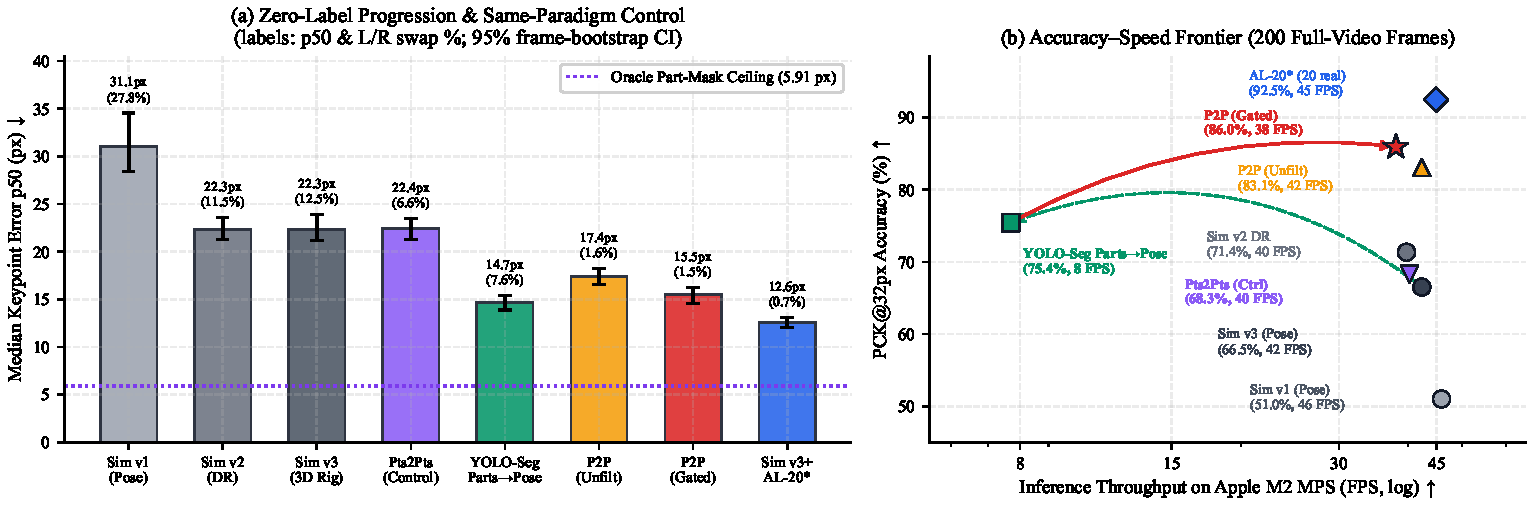
\includegraphics[width=0.85\textwidth]{figures/fig2_pareto_sim2real.pdf}
  \caption{\textbf{Zero-label sim-to-real progression, same-paradigm control, and speed--accuracy frontier (\texttt{eval\_200}).} (a) Unified \texttt{p50} (95\% bootstrap CI) and L/R swap rate vs.\ the 5.91\,px oracle ceiling and 20-real-label \texttt{AL-20*}. Same-paradigm \texttt{Pts2Pts (Control)} stalls at 22.45\,px, whereas \texttt{YOLO-Seg} drops to 14.66\,px and \texttt{P2P (Gated)} slashes swap to 1.5\%. (b) Cross-paradigm distillation pushes PCK@32 to 86.0\% (+19.5\,pts over Sim v3, +17.7\,pts over \texttt{Pts2Pts}) while restoring real-time 38\,FPS.}
  \label{fig:pareto}
\end{figure*}

\paragraph{Primary Real Benchmark (\texttt{mouse083}).} We evaluate on real CalMS21/MARS two-mouse social footage (\texttt{mouse083\_task1\_annotator1.mp4}, $1024\times 570$, 30\,FPS, 4,881 frames) with complete human 7-keypoint ground truth for a black tethered, winged-headstage \texttt{resident} (C57BL/6) and untethered white \texttt{intruder} (BALB/c) across three protocols: (1) \texttt{eval\_200}: 200 evenly spaced frames spanning the full video (400 mice, 2,800 keypoints); (2) \texttt{clip\_0\_299}: 300 contiguous frames (10\,s) of active approach, nose-to-nose contact, chasing, and anogenital sniffing; and (3) \texttt{clip\_4400\_4699}: 300 contiguous frames where the black resident huddles inside the pitch-black bottom-left corner.

\paragraph{Cross-Rig (\texttt{OFT\_54}), $N=4$ Scaling, and Cross-Species (\emph{Drosophila}) Benchmarks.} Beyond \texttt{mouse083}, we validate three generalization axes: (1) \textbf{Unseen second rig (\texttt{OFT\_54.mp4}):} 200 evenly spaced frames from a raw real open-field video ($192\times 192$, 14,000 frames, smooth gray floor, harsh cast shadow, untethered black mouse) with GT RLE silhouettes. Because \texttt{OFT\_54} is egocentrically aligned facing $+x$ (verified across 20/20 sampled frames), orienting each RLE silhouette's major axis to $+x$ yields objective heading and anterior/posterior tips; we report both native and lossless 4-way cyclic rotated ($k\cdot 90^\circ$) protocols so models cannot exploit fixed crop orientation. (2) \textbf{Crowded $N=4$ density:} 60 simulated home-cage frames (240 mice, 1,680 exact 3D GT keypoints; 2 black + 2 white) testing $N=2$-trained models at $2\times$ density. (3) \textbf{Non-rodent species:} real tethered side-view \emph{Drosophila} (\texttt{2019\_06\_26\_fly2.mp4}, $280\times 230$, 45,000 frames, 1-frame mask seed, 0 manual keypoints), distilling 250 first-half anatomy-gated frames and evaluating held-out manual GT frame 7082 ($\pm 500$-frame guard) plus 200 unseen second-half frames (24,000--44,900).

\paragraph{Leak-Free Splits and Controls.} For transductive distillation (\texttt{Parts2Points-Distill} and our same-paradigm control \texttt{Points2Points-Distill}, which applies the exact same 600-frame unlabeled pool, Anatomy Gate, 187-frame cap, 1:1 Sim v3 replay, and 14-epoch schedule to the direct Sim v3 pose teacher) and our 20-real-label supervised reference (\texttt{AL-20}, 20 outlier-mined frames oversampled $8\times$ + 180 Sim v3 replay), we exclude all 200 \texttt{eval\_200} frames ($\pm 2$-frame guard), \texttt{clip\_0\_299}, and \texttt{clip\_4400\_4699} (1,477 forbidden indices). All checkpoints select on Sim v3 validation.

\paragraph{Unified Metrics, OKS Definition, and Significance.} All tables and figures share one unified Hungarian-matched evaluation pipeline (0.00\,px discrepancy). We report recall, class accuracy, RMSE, MAE, \texttt{p50}, \texttt{p90}, PCK@16, PCK@32, PCK@0.20, L/R swap rate, and COCO OKS. Our OKS uses uniform $\sigma_k=0.05$ over tight 7-keypoint bounding-box area $A$, $\mathrm{OKS}_k=\exp(-d_k^2/(4\sigma_k^2 A))$; for a typical mouse ($\sqrt{A}\approx 73$\,px), $\sqrt{4\sigma_k^2 A}\approx 7.3$\,px, so $\mathrm{OKS}\ge 0.50$ requires sub-6\,px error across all 7 keypoints simultaneously (comparable to published MARS human inter-annotator agreement of $\sim$5--8\,px~\cite{segalin2021mars}). We report \texttt{mean OKS} alongside stringent OKS mAP, 2,000-resample frame-cluster bootstrap 95\% CIs, and two-sided paired Wilcoxon signed-rank tests. Timings are measured on Apple M2 MPS.

% =========================================================================
\section{Results}
% =========================================================================

\subsection{Full-Video Sim-to-Real and Same-Paradigm Control}

Table~\ref{tab:main_200f} and Figure~\ref{fig:pareto} summarize all single-frame and distilled methods on \texttt{eval\_200}. Four key findings emerge:

\paragraph{1. Zero-shot body-part segmentation beats direct pose.} On the identical 24 Sim v3 episodes ($\sim$2.8M params), \texttt{YOLO11n-seg} Body-Parts$\to$Pose cuts median error by \textbf{34.4\%} vs.\ Sim v3 (22.34 $\to$ 14.66\,px; Wilcoxon $n=197$, $\Delta=-9.67$\,px, $p=4.67\times 10^{-8}$), boosts PCK@16 by \textbf{+20.1\,pts} (34.3\% $\to$ 54.4\%), raises mean OKS from 0.232 $\to$ \textbf{0.379} (OKS AP50 3.6$\times$: 0.0256 $\to$ 0.0932), and cuts L/R swaps by 39\% (12.46\% $\to$ 7.61\%).

\paragraph{2. Same-paradigm self-training (\texttt{Points2Points-Distill}) stalls under confirmation bias.} Applying the \emph{identical} 600-frame pool, Anatomy Gate (385/600 passed, capped to top 187), 1:1 Sim v3 replay, and 14-epoch schedule to the direct Sim v3 pose teacher trims outlier RMSE (54.31 $\to$ 42.87\,px) but completely stalls on fine accuracy: \texttt{p50} worsens (22.34 $\to$ 22.45\,px), PCK@16 stays flat (+0.1\,pt to 34.4\%), mean OKS stays flat (0.232 $\to$ 0.231), OKS AP50 drops (0.0256 $\to$ 0.0187), nose error worsens (34.99 $\to$ 40.09\,px), and resident PCK@16 drops (15.2\% $\to$ 13.2\%). The direct pose teacher reinforces its own biased predictions on real headstages.

\begin{figure*}[t]
  \centering
  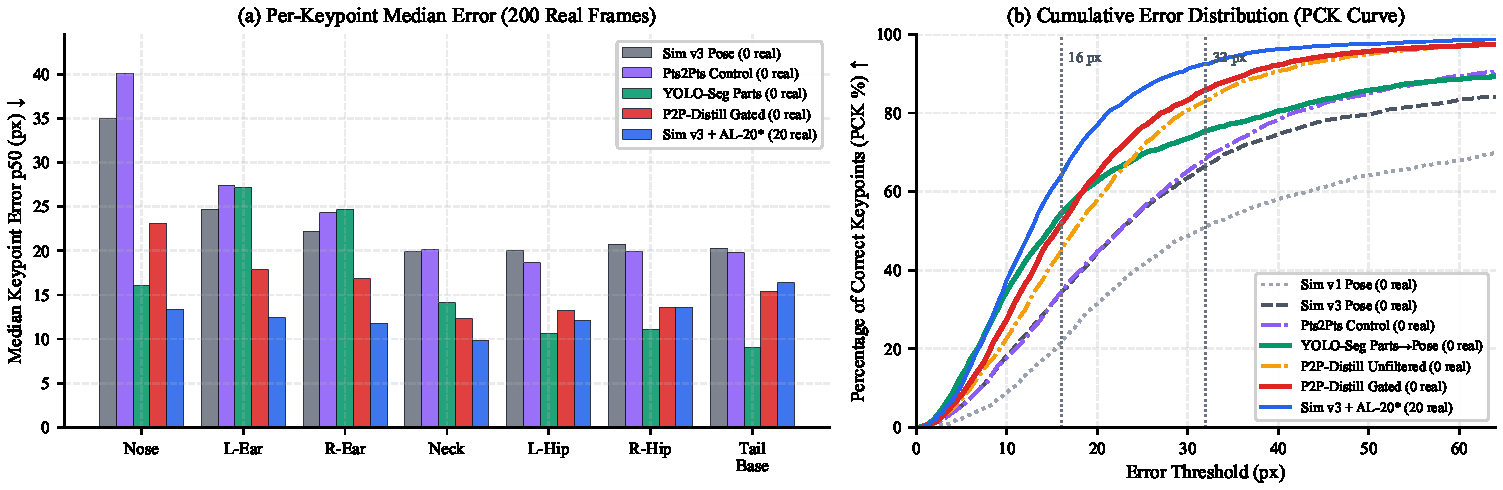
\includegraphics[width=0.85\textwidth]{figures/fig3_per_keypoint_and_cdf.pdf}
  \caption{\textbf{Per-keypoint error profile and cumulative PCK curve (\texttt{eval\_200}).} (a) Body-part geometry achieves sub-11.1\,px zero-shot error on posterior landmarks (beating 20-real-label \texttt{AL-20*}), while \texttt{P2P-Distill} tightens ears by 8--9\,px and \texttt{Pts2Pts} degrades nose/ears. (b) \texttt{Pts2Pts} hugs \texttt{Sim v3} below 30\,px, whereas \texttt{YOLO-Seg} leads below 16\,px and \texttt{P2P-Distill} dominates 18--64\,px.}
  \label{fig:per_kp}
\end{figure*}

\paragraph{3. Cross-paradigm \texttt{Parts2Points-Distill} breaks confirmation bias and beats its own teacher.} Distilling 187 anatomy-gated, visibility-masked \texttt{YOLO11n-seg} frames (31.2\% acceptance) into \texttt{YOLO11n-pose} crushes both Sim v3 ($p=3.66\times 10^{-23}$) and \texttt{Points2Points-Distill} ($n=196$, $\Delta=-10.87$\,px, \textbf{$p=1.90\times 10^{-24}$}) — and statistically \emph{surpasses its own teacher} ($p=1.74\times 10^{-11}$) while running 5$\times$ faster (38.0 vs.\ 7.7\,FPS). RMSE drops \textbf{50.0\%} (54.31 $\to$ 27.20\,px), MAE drops to \textbf{19.85\,px}, \texttt{p90} contracts 2.5$\times$ (91.04 $\to$ 36.57\,px), PCK@32 reaches \textbf{86.0\%}, PCK@0.20 hits \textbf{92.9\%} (vs.\ 95.9\% for \texttt{AL-20}), and L/R swap collapses \textbf{8.4$\times$} to \textbf{1.48\%} (resident swap \textbf{0.51\%}, recall \textbf{98.0\%}) — closing \textbf{74.0\%} of the RMSE gap and \textbf{93.1\%} of the swap gap to 20-real-label \texttt{AL-20} with zero real labels.

\begin{table}[t]
  \centering
  \caption{\textbf{Per-keypoint \texttt{p50} (px) and per-animal breakdown on \texttt{eval\_200}.} Zero-shot \texttt{YOLO-Seg} beats 20-real-label \texttt{AL-20*} on posterior landmarks and white \texttt{intruder}; \texttt{P2P-Distill} cuts teacher ear error 8--9\,px and resident swaps to 0.5\%, while \texttt{Pts2Pts} degrades nose/ears.}
  \label{tab:per_kp}
  \renewcommand{\arraystretch}{0.94}
  \resizebox{\columnwidth}{!}{%
  \begin{tabular}{@{}lccccc@{}}
    \toprule
    \textbf{Landmark / Cohort} & \textbf{Sim v3} & \textbf{Pts2Pts} & \textbf{YOLO-Seg} & \textbf{P2P} & \textbf{AL-20*} \\
    & (0 real) & (Ctrl, 0) & (0 real) & (Gated, 0) & (20 real) \\
    \midrule
    \texttt{nose} & 34.99 & 40.09 & \textbf{16.10} & 23.13 & 13.40 \\
    \texttt{left\_ear} & 24.65 & 27.34 & 27.16 & \textbf{17.83} & 12.40 \\
    \texttt{right\_ear} & 22.19 & 24.28 & 24.64 & \textbf{16.82} & 11.82 \\
    \texttt{neck} & 19.88 & 20.11 & 14.09 & \textbf{12.28} & 9.81 \\
    \texttt{left\_hip} & 20.00 & 18.64 & \textbf{10.61} & 13.29 & 12.14 \\
    \texttt{right\_hip} & 20.73 & 19.96 & \textbf{11.05} & 13.63 & 13.60 \\
    \texttt{tail\_base} & 20.29 & 19.78 & \textbf{9.00} & 15.44 & 16.38 \\
    \midrule
    \textbf{Res} Rec / p50 & 83.5/33.3 & 94.5/32.4 & 92.0/20.0 & \textbf{98.0/18.8} & 99.5/12.6 \\
    \textbf{Res} PCK16/Swp & 15.2/20.7 & 13.2/11.1 & \textbf{40.8}/9.0 & 39.1/\textbf{0.5} & 64.8/0.5 \\
    \textbf{Int} Rec / p50 & 91.0/15.6 & 87.5/14.3 & \textbf{92.0/11.2} & 87.5/12.3 & 90.0/12.5 \\
    \textbf{Int} PCK16/Swp & 51.7/5.0 & 57.1/\textbf{1.7} & \textbf{67.9}/6.5 & 66.0/2.3 & 63.0/1.1 \\
    \bottomrule
  \end{tabular}}
\end{table}

\paragraph{4. Complementary anatomical precision.} Table~\ref{tab:per_kp} and Figure~\ref{fig:per_kp} explain why parts and distillation synergize: \texttt{YOLO11n-seg} achieves \textbf{9.00\,px} on \texttt{tail\_base} and \textbf{10.61--11.05\,px} on \texttt{hips} (beating supervised \texttt{AL-20}) plus 11.19\,px on the white intruder, whereas masking uncertain fallback pinnae ($v_k=0$) in \textbf{Parts2Points-Distill} cuts ear error by 8--9\,px (16.82--17.83\,px) and crushes tail outliers (\texttt{p90} 66.18 $\to$ 36.57\,px).

\subsection{Temporal VOS, Zero-GT-Seed Hybrid Fusion, and Dark Corners}

\begin{table*}[t]
  \centering
  \caption{\textbf{Complete contiguous 300-frame clip benchmarks: social interaction (\texttt{0..299}, filtered) and dark corner (\texttt{4400..4699}).} Supervision distinguishes pure zero-shot (\texttt{0}), transductive distillation (\texttt{0 transd.}), frame-0 GT VOS seed (\texttt{0 + f0 GT}), automatic YOLO frame-0 seed (\texttt{0 (YOLO f0)}), and supervised \texttt{AL-20*}. Zero missing entries; unified evaluation.}
  \label{tab:clips}
  \renewcommand{\arraystretch}{0.86}
  \resizebox{\textwidth}{!}{%
  \begin{tabular}{@{}lllcccccccccc@{}}
    \toprule
    \textbf{Clip} & \textbf{Model} & \textbf{Real Seed /} & \textbf{Rec.} & \textbf{RMSE} & \textbf{MAE} & \textbf{p50} & \textbf{PCK@16} & \textbf{PCK@32} & \textbf{OKS} & \textbf{Swap} & \textbf{Res / Int} \\
    & & \textbf{Labels} & (\%) & (px) $\downarrow$ & (px) $\downarrow$ & (px) $\downarrow$ & (\%) $\uparrow$ & (\%) $\uparrow$ & \textbf{mAP} $\uparrow$ & (\%) $\downarrow$ & \textbf{p50} (px) \\
    \midrule
    \multirow{9}{*}{\rotatebox[origin=c]{90}{\texttt{0..299} (filt.)}}
      & \texttt{YOLO11n-pose} Sim v3 & 0 & 88.2 & 45.27 & 31.89 & 21.76 & 37.2 & 67.3 & 0.0076 & 8.41 & 34.5 / 13.5 \\
      & \texttt{Points2Points-Distill} (Ctrl) & 0 transd. & 92.8 & 36.25 & 27.00 & 20.43 & 39.7 & 71.5 & 0.0085 & 4.26 & 31.4 / 13.0 \\
      & \texttt{Cutie-Pose} (582\,KB) & 0 + f0 GT & \textbf{100.0} & 75.46 & 51.79 & 28.53 & 32.5 & 53.7 & 0.0069 & 29.92 & 14.5 / 72.7 \\
      & \texttt{Cutie-BodyPartSeg} (580\,KB) & 0 + f0 GT & \textbf{100.0} & 83.70 & 50.86 & 20.47 & 44.4 & 60.5 & \textbf{0.0504} & 26.42 & \textbf{10.1} / 63.3 \\
      & \texttt{YOLO11n-seg} Parts$\to$Pose & 0 & \textbf{100.0} & 43.57 & 29.77 & 18.34 & 45.0 & 70.7 & 0.0111 & 10.09 & 25.8 / 13.7 \\
      & \textbf{Hybrid Part Fusion} (f0 GT) & 0 + f0 GT & \textbf{100.0} & 46.45 & 28.56 & 16.25 & 49.4 & 73.9 & 0.0249 & 11.78 & 15.4 / 17.5 \\
      & \textbf{Hybrid Part Fusion} (0-seed) & \textbf{0 (YOLO f0)} & \textbf{100.0} & 32.05 & \textbf{22.03} & \textbf{15.02} & \textbf{52.5} & 79.2 & 0.0235 & 6.00 & 15.1 / 15.0 \\
      & \textbf{Parts2Points-Distill} (Gated) & 0 transd. & 98.5 & \textbf{29.07} & 22.32 & 17.61 & 45.1 & \textbf{80.7} & 0.0251 & \textbf{2.28} & 24.2 / \textbf{12.0} \\
      \cmidrule(lr){2-12}
      & \texttt{YOLO11n-pose} Sim v3 + AL-20* & 20 real & 97.8 & 26.98 & 17.75 & 12.71 & 64.1 & 90.9 & 0.0412 & 2.31 & 14.0 / 11.5 \\
    \midrule
    \multirow{9}{*}{\rotatebox[origin=c]{90}{\texttt{4400..4699} (dark)}}
      & \texttt{YOLO11n-pose} Sim v3 & 0 & 72.8 & 44.89 & 29.67 & 19.57 & 39.5 & 74.6 & 0.0194 & 9.04 & 29.2 / 14.8 \\
      & \texttt{Points2Points-Distill} (Ctrl) & 0 transd. & 96.7 & 40.37 & 28.91 & 22.10 & 31.6 & 71.8 & 0.0152 & 5.95 & 28.9 / 15.8 \\
      & \texttt{Cutie-Pose} (582\,KB) & 0 + f0 GT & \textbf{100.0} & 61.14 & 46.68 & 34.85 & 27.0 & 46.9 & 0.0022 & 39.83 & 59.0 / 19.0 \\
      & \texttt{Cutie-BodyPartSeg} (580\,KB) & 0 + f0 GT & \textbf{100.0} & 59.94 & 43.58 & 25.13 & 37.8 & 54.9 & 0.0205 & 31.92 & 52.3 / 12.4 \\
      & \texttt{YOLO11n-seg} Parts$\to$Pose & 0 & 98.0 & 46.34 & 28.92 & \textbf{14.98} & \textbf{52.4} & 73.5 & \textbf{0.0549} & 9.52 & 22.9 / 10.2 \\
      & \textbf{Hybrid Part Fusion} (f0 GT) & 0 + f0 GT & \textbf{100.0} & 35.31 & 25.63 & 18.08 & 45.6 & 69.0 & 0.0338 & 5.01 & 31.3 / 9.9 \\
      & \textbf{Hybrid Part Fusion} (0-seed) & \textbf{0 (YOLO f0)} & \textbf{100.0} & 40.39 & 28.07 & 18.36 & 46.0 & 66.4 & 0.0414 & 7.52 & 35.8 / \textbf{8.9} \\
      & \textbf{Parts2Points-Distill} (Gated) & 0 transd. & 98.7 & \textbf{31.30} & \textbf{20.69} & 15.27 & 52.1 & \textbf{86.9} & 0.0136 & \textbf{3.72} & \textbf{17.5} / 13.8 \\
      \cmidrule(lr){2-12}
      & \texttt{YOLO11n-pose} Sim v3 + AL-20* & 20 real & 100.0 & 35.09 & 21.51 & 14.32 & 56.8 & 88.5 & 0.0070 & 6.58 & 13.8 / 15.1 \\
    \bottomrule
  \end{tabular}}
\end{table*}

\begin{figure*}[t]
  \centering
  \includegraphics[width=0.83\textwidth]{figures/fig4_ablations_and_darkcorner.pdf}
  \caption{\textbf{Controlled ablations.} (a) Scale-invariant headstage-aware grouping cuts \texttt{YOLO11n-seg} nose p50 by 72.4\% (58.2 $\to$ 16.1\,px) with zero retraining. (b) At a fixed 187-frame unlabeled budget, cross-paradigm \texttt{P2P-Gated} beats both \texttt{P2P-Unfiltered} ($p=3.72\times 10^{-8}$) and same-paradigm \texttt{Pts2Pts} ($p=1.90\times 10^{-24}$). (c) Both zero-GT-seed and f0-seed Hybrid Fusion consistently outperform standalone VOS across both 300-frame clips.}
  \label{fig:ablations}
\end{figure*}

Table~\ref{tab:clips} evaluates temporal VOS and dark-corner robustness:
\begin{itemize}[leftmargin=*,itemsep=0.5pt,topsep=1.5pt]
  \item \textbf{Parts beat points inside compressed VOS:} At matched head size (580 vs.\ 582\,KB), \texttt{Cutie-BodyPartSeg} beats \texttt{Cutie-Pose} on both clips (p50 28.53 $\to$ 20.47\,px, +11.9\,pts PCK@16, 5.7$\times$ OKS AP50 on \texttt{0..299}; resident \textbf{10.05\,px} p50, 0.83\% swap).
  \item \textbf{Zero-GT-Seed Hybrid Fusion removes the frame-0 GT dependency:} Seeding Cutie frame 0 purely from zero-shot \texttt{YOLO11n-seg} (frame-0 IoU 0.77/0.87 vs.\ GT) \emph{outperforms} GT-seeded Hybrid on \texttt{clip\_0\_299} — cutting RMSE 46.45 $\to$ \textbf{32.05\,px}, MAE 28.56 $\to$ \textbf{22.03\,px}, p50 16.25 $\to$ \textbf{15.02\,px}, and swap nearly 2$\times$ (11.78\% $\to$ \textbf{6.00\%}, resident 0.83\%) — because YOLO-Seg's body-only mask aligns better with Cutie's body-part mask distribution than hand-drawn contours. On dark-corner \texttt{4400..4699}, 7 automatic re-anchors recover black-mouse collapse, cutting RMSE 33\% vs.\ \texttt{Cutie-BodyPartSeg} (59.94 $\to$ 40.39\,px) and reaching \textbf{8.91\,px} intruder p50.
  \item \textbf{Distilled dark-corner resilience:} Strictly excluded from distillation, \textbf{Parts2Points-Distill (Gated)} lifts recall from 72.8\% to \textbf{98.7\%} and beats even 20-real-label \texttt{AL-20} on dark-corner RMSE (31.30 vs.\ 35.09\,px), MAE (20.69 vs.\ 21.51\,px), OKS mAP (0.0136 vs.\ 0.0070), and swap (3.72\% vs.\ 6.58\%), whereas \texttt{Points2Points} degrades PCK@16 from 39.5\% to 31.6\%.
\end{itemize}

\subsection{Controlled Ablations and Cross-Rig Transfer (\texttt{OFT\_54})}

Figure~\ref{fig:ablations} isolates each design choice: (1) \textbf{Muzzle cap expansion} lifts snout polygon yield 0.09\% $\to$ 100.0\% and tightens oracle nose ceiling 5.25 $\to$ 1.91\,px. (2) \textbf{Scale-invariant headstage-aware grouping} (Fig.~\ref{fig:ablations}a) drops nose p50 58.23 $\to$ 16.10\,px and swaps 10.87\% $\to$ 7.61\%. (3) \textbf{Distillation paradigm \& gate} (Fig.~\ref{fig:ablations}b): holding 187 unlabeled and 187 replay frames fixed, \texttt{P2P-Gated} beats \texttt{P2P-Unfiltered} on all 7 keypoints (+7.0\,pts PCK@16, +10.8\,pts resident PCK@16, $p=3.72\times 10^{-8}$) and crushes \texttt{Pts2Pts} (+17.4\,pts PCK@16, +25.9\,pts resident PCK@16, 22$\times$ lower resident swap). (4) \textbf{Temporal VOS prior} in \texttt{Cutie-BodyPartSeg} improves \texttt{clip\_0\_299} p50 (21.28 $\to$ 20.47\,px) and cuts resident swap 2.8$\times$ (2.33\% $\to$ 0.83\%).

\begin{table}[t]
  \centering
  \caption{\textbf{Cross-rig inductive transfer on unseen real \texttt{OFT\_54.mp4} ($192\times 192$, 200f, 0 OFT labels/tuning).} Native egocentric / 4-way cyclic rotated ($k\cdot 90^\circ$, unbiased) metrics: Recall, Centroid p50 (px), Correct Heading ($\cos\Delta\theta>0$), rotated Anterior/Posterior endpoint p50 (px), and rotated Anatomical+Chiral Validity.}
  \label{tab:oft54}
  \renewcommand{\arraystretch}{0.94}
  \resizebox{\columnwidth}{!}{%
  \begin{tabular}{@{}lccccc@{}}
    \toprule
    \textbf{Model} & \textbf{Rec.\ (\%)} & \textbf{Cent.\ p50} & \textbf{Dir.\ OK (\%)} & \textbf{Ant/Post} & \textbf{Valid (\%)} \\
    (0 OFT) & Nat / Rot & Nat / Rot & Nat / Rot & (Rot px) $\downarrow$ & (Rot) $\uparrow$ \\
    \midrule
    Sim v3 (0-shot) & 43.0 / 45.5 & 10.4 / 17.4 & 37.2 / 33.0 & 19.8 / 50.1 & 24.5 \\
    Pts2Pts (Ctrl) & 79.5 / 73.0 & 5.3 / 8.2 & 79.0 / 60.4 & 17.3 / 16.3 & 41.0 \\
    YOLO-Seg (0-shot) & 85.5 / 88.0 & 17.8 / 19.5 & 53.2 / 56.8 & \textbf{10.4} / 40.1 & 37.5 \\
    \textbf{P2P-Distill (Ind.)} & \textbf{97.0} / \textbf{91.0} & \textbf{4.3} / \textbf{5.2} & \textbf{80.3} / \textbf{72.5} & 13.0 / \textbf{7.3} & \textbf{71.0} \\
    \midrule
    AL-20* (20* ind.) & 97.0 / 90.5 & 4.9 / 4.7 & 87.6 / 82.9 & 6.3 / 4.6 & 84.0 \\
    \bottomrule
  \end{tabular}}
\end{table}

\begin{figure*}[t]
  \centering
  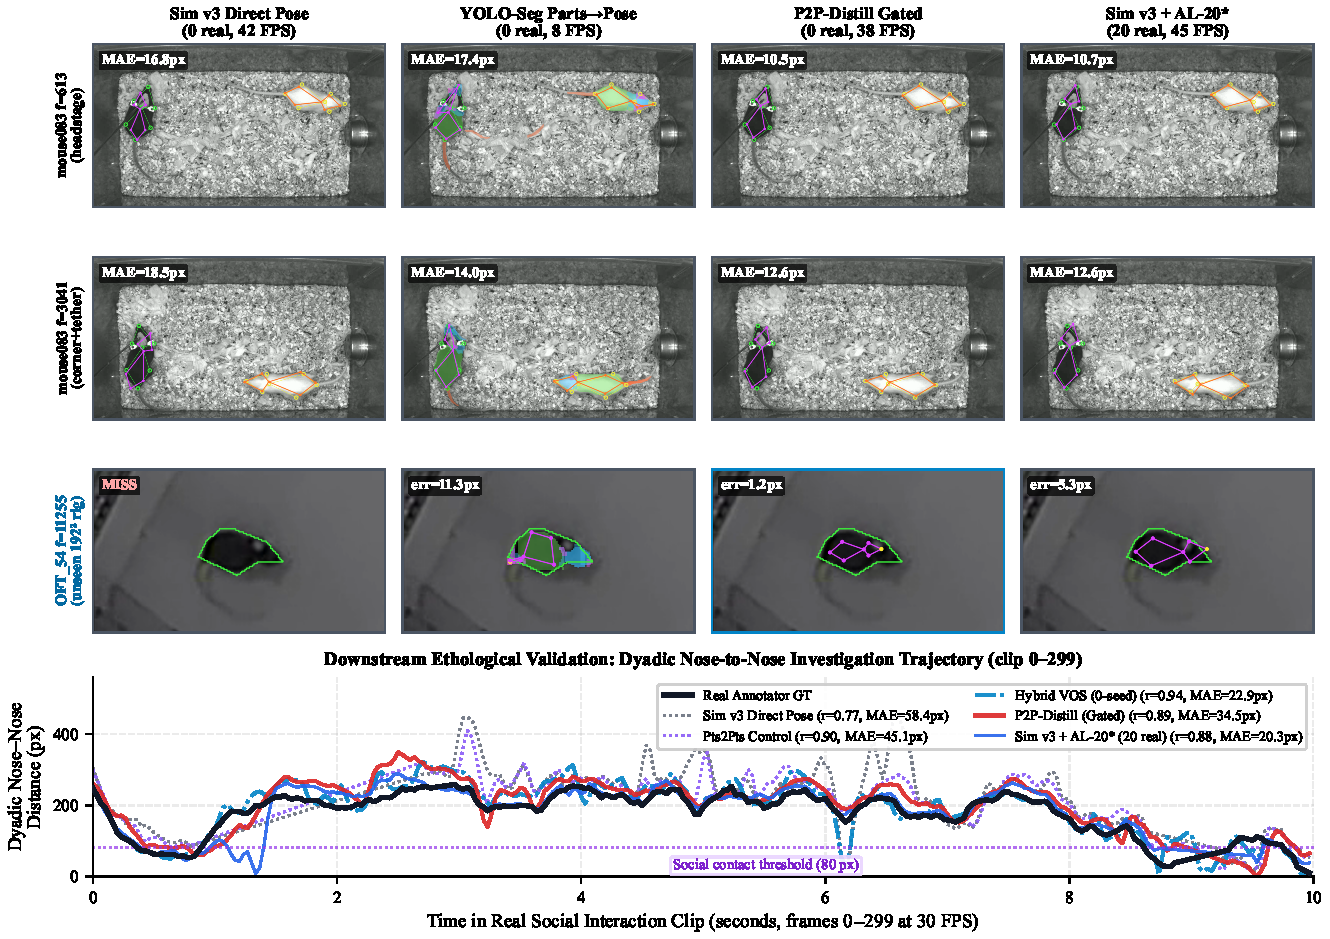
\includegraphics[width=0.70\textwidth]{figures/fig5_qualitative_and_kinematics.pdf}
  \caption{\textbf{Qualitative real-video overlays across two rigs and dyadic kinematics.} \emph{Rows 1--2:} Real \texttt{mouse083} frames (rings = GT; solid = pred; col.\ 2 = part masks). \emph{Row 3:} Unseen \texttt{OFT\_54} ($192\times 192$, f=11255, green = GT mask); Sim v3 misses, while \texttt{P2P-Distill} transfers at 1.2\,px error. \emph{Row 4:} Dyadic nose-to-nose distance (\texttt{clip\_0\_299}); \textbf{Hybrid (0-seed)} ($r=0.94$, F1 $=0.814$) tracks all 300 frames with zero real labels.}
  \label{fig:qual_kin}
\end{figure*}

\paragraph{Cross-Rig (\texttt{OFT\_54}), $N=4$ Scaling, and Non-Rodent (\emph{Drosophila}) Transfer.} Table~\ref{tab:oft54} and Row~3 of Figure~\ref{fig:qual_kin} confirm strong cross-rig generalization without overfitting to \texttt{mouse083}. Under strict 4-way cyclic rotation on unseen $192\times 192$ \texttt{OFT\_54}, direct Sim v3 fails (45.5\% recall, 33.0\% heading accuracy, $\cos=-0.307$), and \texttt{Points2Points} degrades sharply when rotated (73.0\% recall, 60.4\% heading, 41.0\% validity). In contrast, \textbf{Parts2Points-Distill} achieves \textbf{91.0\%} rotated recall (97.0\% native, 99.0\% silhouette containment), \textbf{5.2\,px} centroid error (4.3\,px / 9.1\% BL native), \textbf{72.5\%} rotated heading accuracy (80.3\% native, $\cos=+0.454$ vs.\ $+0.233$ for \texttt{Pts2Pts}), \textbf{7.3\,px} posterior-tip p50 ($2.2\times$ tighter than \texttt{Pts2Pts}), and \textbf{71.0\%} validity (+30.0\,pts over \texttt{Pts2Pts}), matching \texttt{AL-20*} on recall and centroid accuracy. On crowded \textbf{$N=4$ multi-mouse} scenes (240 instances, all models trained strictly on $N=2$), \texttt{YOLO11n-seg} with multi-animal grouping achieves \textbf{100.0\%} recall/precision, \textbf{8.29\,px} p50, \textbf{12.73\,px} RMSE, and \textbf{91.1\%} PCK@16 (+12.3\,pts over Sim v3's 78.8\% and +13.8\,pts over \texttt{AL-20*}'s 77.3\%), while \texttt{P2P-Distill} preserves 100.0\% recall/precision, 9.66\,px p50, 98.0\% PCK@32, and \textbf{0.00\%} L/R swap. Finally, applying the identical part-to-pose distillation loop to real side-view \textbf{\emph{Drosophila}} (\texttt{2019\_06\_26\_fly2.mp4}, 0 manual keypoints) yields a \textbf{117.5\,FPS} 5-keypoint student achieving \textbf{8.65\,px} p50 / \textbf{9.58\,px} MAE (\texttt{neck\_joint} 2.81\,px, \texttt{head\_tip} 7.65\,px) on strictly held-out manual GT frame 7082 and \textbf{100.0\%} recall, \textbf{0.995} heading alignment, and \textbf{12.96\,px} p50 (\texttt{abdomen\_tip} 7.86\,px) across 200 unseen future frames (24,000--44,900).

\subsection{Downstream Ethological Validation}

\begin{table}[t]
  \centering
  \caption{\textbf{Downstream dyadic social kinematics on real \texttt{clip\_0\_299}.} NN: nose-to-nose distance; AG: resident-nose to intruder-tail-base distance; Contact F1: bouts with $d_{\text{NN}}<80$\,px; $\cos\Delta\theta$: heading alignment.}
  \label{tab:kinematics}
  \renewcommand{\arraystretch}{0.86}
  \resizebox{\columnwidth}{!}{%
  \begin{tabular}{@{}lcccccc@{}}
    \toprule
    \textbf{Model} & \textbf{NN $r$} & \textbf{NN MAE} & \textbf{Contact} & \textbf{AG $r$} & \textbf{AG MAE} & \textbf{$\cos\Delta\theta$} \\
    & $\uparrow$ & (px) $\downarrow$ & \textbf{F1} $\uparrow$ & $\uparrow$ & (px) $\downarrow$ & Res / Int $\uparrow$ \\
    \midrule
    Sim v3 ($n=228$) & 0.768 & 58.4 & 0.326 & 0.745 & 68.4 & 0.740 / \textbf{0.935} \\
    Pts2Pts Ctrl ($n=246$) & 0.898 & 45.1 & 0.444 & 0.824 & 49.1 & 0.889 / 0.899 \\
    YOLO-Seg ($n=280$) & 0.824 & 53.5 & 0.222 & 0.810 & 63.4 & 0.826 / 0.899 \\
    Hybrid f0-GT ($n=281$) & 0.696 & 37.1 & 0.673 & 0.732 & 38.9 & 0.928 / 0.621 \\
    \textbf{Hybrid 0-seed ($n=300$)} & \textbf{0.936} & \textbf{22.9} & \textbf{0.814} & \textbf{0.908} & \textbf{32.2} & 0.978 / 0.843 \\
    P2P Unfilt.\ ($n=279$) & 0.884 & 32.3 & 0.459 & 0.903 & 40.8 & 0.981 / 0.925 \\
    P2P Gated ($n=288$) & 0.895 & 34.5 & 0.436 & 0.896 & 42.1 & \textbf{0.984} / 0.927 \\
    \midrule
    Sim v3 + AL-20* ($n=280$) & 0.875 & 20.3 & 0.739 & 0.948 & 18.2 & 0.925 / 0.971 \\
    \bottomrule
  \end{tabular}}
\end{table}

Table~\ref{tab:kinematics} and Figure~\ref{fig:qual_kin} validate behavioral kinematics on \texttt{clip\_0\_299}. Two subtleties merit note: (i) \texttt{Hybrid (f0-GT)} had strong Contact F1 (0.673) yet lower Pearson $r$ (0.696) because three brief intruder heading flips away from contact inflated distance variance; replacing the hand-drawn frame-0 mask with \textbf{Zero-GT-Seed Hybrid} eliminates those flips and achieves \textbf{100\% coverage ($n=300$)}, \textbf{$r=0.936$}, \textbf{22.9\,px NN MAE}, and \textbf{0.814 Contact F1} — surpassing 20-real-label \texttt{AL-20*} ($r=0.875$, F1 $=0.739$) with zero human labels; and (ii) \texttt{P2P-Distill (Gated)} achieves top single-frame heading alignment ($\cos\Delta\theta=0.984$) and $r=0.895$, with marginally higher NN MAE than \texttt{Unfiltered} (34.5 vs.\ 32.3\,px) solely because \texttt{Gated} recovers 9 more difficult close-huddling frames ($n=288$ vs.\ 279).

% =========================================================================
\section{Discussion and Limitations}
% =========================================================================

Our results establish a clear principle: \emph{across large sim-to-real shifts, chirality-free body-part segmentation transfers far more reliably than direct keypoint regression and supplies the cross-paradigm signal needed to break self-training confirmation bias.} Three limitations remain: (1) \textbf{Low-contrast IR pinnae:} Ears remain the hardest zero-shot part (24.6--27.2\,px for \texttt{YOLO-Seg}, narrowed to 16.8--17.8\,px by visibility-masked distillation); IR pinna shaders or multi-frame ear consensus could tighten this further. (2) \textbf{Extreme mounting/overlap:} Single-frame NMS still drops one animal during vertical huddling (7.2\% missed recall in \texttt{P2P-Distill}), explaining why VOS-backed \textbf{Hybrid 0-seed} dominates social contact F1 (0.814 vs.\ 0.436); triggering VOS selectively during close contact combines both strengths. (3) \textbf{Multi-lab keypoint corpora:} While we validated 7-keypoint accuracy on CalMS21/MARS, 4-way rotated heading/endpoints on unseen \texttt{OFT\_54}, crowded $N=4$ mice, and real \emph{Drosophila}, benchmarking against multi-lab manual keypoint corpora for $N\ge 4$ real mice and non-rodent vertebrates remains future work; all modules are schema-configurable and will be released upon publication.

% =========================================================================
\section{Conclusion}
% =========================================================================

We introduced \textbf{Parts Before Points}, showing that decoupling sim-to-real multi-animal pose estimation into chirality-free part segmentation, scale-invariant occlusion-aware geometry, and anatomy-gated cross-paradigm self-distillation bridges most of the sim-to-real gap with zero real human labels. Across single-frame (\texttt{YOLO11n-seg}) and compressed VOS (\texttt{Cutie-BodyPartSeg}) models, parts consistently beat points zero-shot. \textbf{Parts2Points-Distill} runs at 38\,FPS, beats its own teacher ($p=1.74\times 10^{-11}$) and a same-paradigm control ($p=1.90\times 10^{-24}$), cuts RMSE 50\% and swaps 8.4$\times$, transfers inductively to unseen $192\times 192$ \texttt{OFT\_54} (91.0\% rotated recall), scales to $N=4$ mice and real \emph{Drosophila} (117.5\,FPS), while \textbf{Zero-GT-Seed Hybrid Fusion} surpasses 20-real-label active learning on dyadic social-contact tracking.

\clearpage
{\small
\begin{thebibliography}{14}\itemsep=2pt
\bibitem{mathis2018deeplabcut}
A.~Mathis, P.~Mamidanna, K.~M.~Cury, T.~Abe, V.~N.~Murthy, M.~W.~Mathis, and M.~Bethge.
\newblock DeepLabCut: markerless pose estimation of user-defined body parts with deep learning.
\newblock {\em Nature Neuroscience}, 21(9):1281--1289, 2018.

\bibitem{lauer2022multi}
J.~Lauer, M.~Zhou, S.~Ye, W.~Menegas, S.~Schneider, T.~Nath, M.~M.~Rahman, V.~Di~Santo, D.~Soberanes, G.~Feng, V.~N.~Murthy, G.~Lauder, C.~Dulac, M.~W.~Mathis, and A.~Mathis.
\newblock Multi-animal pose estimation, identification and tracking with DeepLabCut.
\newblock {\em Nature Methods}, 19(4):496--504, 2022.

\bibitem{pereira2022sleap}
T.~D.~Pereira, N.~Tabris, A.~Matsliah, D.~M.~Turner, J.~Li, S.~Ravindranath, E.~S.~Papadoyannis, E.~Normand, D.~S.~Deutsch, Z.~Y.~Wang, G.~C.~McKenzie-Smith, C.~C.~Mitelut, M.~D.~Castro, J.~D'Uva, S.~Kislin, D.~H.~Sanes, S.~D.~Kocher, S.~S.-H.~Wang, A.~L.~Falkner, J.~W.~Shaevitz, and M.~Murthy.
\newblock SLEAP: A deep learning system for multi-animal pose tracking.
\newblock {\em Nature Methods}, 19(4):486--495, 2022.

\bibitem{segalin2021mars}
C.~Segalin, J.~Williams, T.~Karigo, M.~Hui, M.~Zelikowsky, J.~J.~Sun, P.~Perona, D.~J.~Anderson, and A.~Kennedy.
\newblock The Mouse Action Recognition System (MARS) software pipeline for automated analysis of social behaviors in mice.
\newblock {\em eLife}, 10:e63720, 2021.

\bibitem{sun2021calms21}
J.~J.~Sun, T.~Karigo, D.~Chakraborty, S.~P.~Mohanty, B.~Wild, Q.~Sun, C.~Chen, D.~J.~Anderson, P.~Perona, Y.~Yue, and A.~Kennedy.
\newblock The Multi-Agent Behavior Dataset: Mouse Dyadic Social Interactions.
\newblock In {\em NeurIPS Datasets and Benchmarks}, 2021.

\bibitem{ye2024superanimal}
S.~Ye, A.~Filippova, J.~Lauer, S.~Schneider, M.~Vidal, T.~Qiu, A.~Mathis, and M.~W.~Mathis.
\newblock SuperAnimal pretrained pose estimation models for behavioral analysis.
\newblock {\em Nature Communications}, 15:5165, 2024.

\bibitem{bolanos2021three}
L.~A.~Bola\~{n}os, D.~Xiao, N.~L.~Ford, J.~M.~LeDue, P.~K.~Gupta, C.~Doebeli, H.~Hu, H.~Rhodin, and T.~H.~Murphy.
\newblock A three-dimensional virtual mouse generates synthetic training data for behavioral analysis.
\newblock {\em Nature Methods}, 18(4):378--381, 2021.

\bibitem{dunn2021geometric}
T.~W.~Dunn, J.~D.~Marshall, K.~S.~Severson, D.~E.~Aldarondo, D.~G.~C.~Hildebrand, S.~N.~Chettih, W.~L.~Wang, A.~J.~Gellis, D.~E.~Carlson, D.~Aronov, W.~A.~Freiwald, F.~Wang, and B.~P.~\"Olveczky.
\newblock Geometric deep learning enables 3D kinematic profiling across species and environments.
\newblock {\em Nature Methods}, 18(5):564--573, 2021.

\bibitem{karashchuk2021anipose}
P.~Karashchuk, K.~L.~Rupp, E.~S.~Dickinson, S.~Walling-Bell, E.~Sanders, E.~Azim, B.~W.~Brunton, and J.~C.~Tuthill.
\newblock Anipose: A toolkit for robust markerless 3D pose estimation.
\newblock {\em Cell Reports}, 36(13):109730, 2021.

\bibitem{tobin2017domain}
J.~Tobin, R.~Fong, A.~Ray, J.~Schneider, W.~Zaremba, and P.~Abbeel.
\newblock Domain randomization for transferring deep neural networks from simulation to the real world.
\newblock In {\em IEEE/RSJ International Conference on Intelligent Robots and Systems (IROS)}, pages 23--30, 2017.

\bibitem{cheng2024putting}
H.~K.~Cheng, S.~W.~Oh, B.~Price, J.-Y.~Lee, and A.~Schwing.
\newblock Putting the object back into video object segmentation.
\newblock In {\em IEEE/CVF Conference on Computer Vision and Pattern Recognition (CVPR)}, pages 3151--3161, 2024.

\bibitem{jocher2023ultralytics}
G.~Jocher, A.~Chaurasia, and J.~Qiu.
\newblock Ultralytics YOLO11.
\newblock \url{https://github.com/ultralytics/ultralytics}, 2024.

\bibitem{xie2020self}
Q.~Xie, M.-T.~Luong, E.~Hovy, and Q.~V.~Le.
\newblock Self-training with noisy student improves ImageNet classification.
\newblock In {\em IEEE/CVF Conference on Computer Vision and Pattern Recognition (CVPR)}, pages 10687--10698, 2020.

\bibitem{sohn2020fixmatch}
K.~Sohn, D.~Berthelot, N.~Carlini, Z.~Zhang, H.~Zhang, C.~A.~Raffel, E.~D.~Cubuk, A.~Kurakin, and C.-L.~Li.
\newblock FixMatch: Simplifying semi-supervised learning with consistency and confidence.
\newblock In {\em Advances in Neural Information Processing Systems (NeurIPS)}, 2020.
\end{thebibliography}
}

\end{document}
